\documentclass{article}

\usepackage{CJKutf8}

\usepackage{listings}
\usepackage{xcolor}
\lstset { %
	language=C++,
	backgroundcolor=\color{black!5}, % set backgroundcolor
	basicstyle=\footnotesize,% basic font setting
}

\usepackage{graphicx} %package to manage images
\graphicspath{ {images/} }

\title{SLAM Theory and Practice: Home Work 2}
\author{Liang Xu \\ liangxucs@gatech.edu}
\date{February 2018}

\begin{document}
\begin{CJK*}{UTF8}{gbsn}
\maketitle

\section{熟悉 Eigen 矩阵运算}
\subsection{在什么条件下,x 有解且唯一?}
Ax = b有解,则|A|不为0. 

\subsection{高斯消元法的原理是什么?}
高斯消元法,是线性代数中的一个算法,可用来求解线性方程组,并可以求出矩阵的秩,以及求出可逆方阵的逆矩阵。高斯消元法会产生出一个“行梯阵式”,阶梯的方式消去对应列的元素,每一次运算能保证消去对应列. 

\subsection{QR 分解的原理是什么?}
对于n阶方阵A,若存在正交矩阵Q和上三角矩阵R,使得A = QR,则该式称为矩阵A的完全QR分解或正交三角分解
\subsection{Cholesky 分解的原理是什么?}
Cholesky 分解是把一个对称正定的矩阵表示成一个下三角矩阵L和其转置的乘积的分解. 它要求矩阵的所有特征值必须大于零,故分解的下三角的对角元也是大于零的. Cholesky分解法又叫平方根法
\begin{figure}[h]
	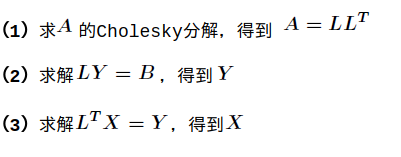
\includegraphics[width=6cm]{cho.png}
	\centering
\end{figure}
\subsection{编程实现 A 为 100 × 100 随机矩阵时,用 QR 和 Cholesky 分解求 x }


\clearpage\end{CJK*}
\end{document}
